% Options for packages loaded elsewhere
\PassOptionsToPackage{unicode}{hyperref}
\PassOptionsToPackage{hyphens}{url}
\PassOptionsToPackage{dvipsnames,svgnames,x11names}{xcolor}
%
\documentclass[
  letterpaper,
  DIV=11,
  numbers=noendperiod]{scrartcl}

\usepackage{amsmath,amssymb}
\usepackage{iftex}
\ifPDFTeX
  \usepackage[T1]{fontenc}
  \usepackage[utf8]{inputenc}
  \usepackage{textcomp} % provide euro and other symbols
\else % if luatex or xetex
  \usepackage{unicode-math}
  \defaultfontfeatures{Scale=MatchLowercase}
  \defaultfontfeatures[\rmfamily]{Ligatures=TeX,Scale=1}
\fi
\usepackage{lmodern}
\ifPDFTeX\else  
    % xetex/luatex font selection
\fi
% Use upquote if available, for straight quotes in verbatim environments
\IfFileExists{upquote.sty}{\usepackage{upquote}}{}
\IfFileExists{microtype.sty}{% use microtype if available
  \usepackage[]{microtype}
  \UseMicrotypeSet[protrusion]{basicmath} % disable protrusion for tt fonts
}{}
\makeatletter
\@ifundefined{KOMAClassName}{% if non-KOMA class
  \IfFileExists{parskip.sty}{%
    \usepackage{parskip}
  }{% else
    \setlength{\parindent}{0pt}
    \setlength{\parskip}{6pt plus 2pt minus 1pt}}
}{% if KOMA class
  \KOMAoptions{parskip=half}}
\makeatother
\usepackage{xcolor}
\setlength{\emergencystretch}{3em} % prevent overfull lines
\setcounter{secnumdepth}{-\maxdimen} % remove section numbering
% Make \paragraph and \subparagraph free-standing
\makeatletter
\ifx\paragraph\undefined\else
  \let\oldparagraph\paragraph
  \renewcommand{\paragraph}{
    \@ifstar
      \xxxParagraphStar
      \xxxParagraphNoStar
  }
  \newcommand{\xxxParagraphStar}[1]{\oldparagraph*{#1}\mbox{}}
  \newcommand{\xxxParagraphNoStar}[1]{\oldparagraph{#1}\mbox{}}
\fi
\ifx\subparagraph\undefined\else
  \let\oldsubparagraph\subparagraph
  \renewcommand{\subparagraph}{
    \@ifstar
      \xxxSubParagraphStar
      \xxxSubParagraphNoStar
  }
  \newcommand{\xxxSubParagraphStar}[1]{\oldsubparagraph*{#1}\mbox{}}
  \newcommand{\xxxSubParagraphNoStar}[1]{\oldsubparagraph{#1}\mbox{}}
\fi
\makeatother


\providecommand{\tightlist}{%
  \setlength{\itemsep}{0pt}\setlength{\parskip}{0pt}}\usepackage{longtable,booktabs,array}
\usepackage{calc} % for calculating minipage widths
% Correct order of tables after \paragraph or \subparagraph
\usepackage{etoolbox}
\makeatletter
\patchcmd\longtable{\par}{\if@noskipsec\mbox{}\fi\par}{}{}
\makeatother
% Allow footnotes in longtable head/foot
\IfFileExists{footnotehyper.sty}{\usepackage{footnotehyper}}{\usepackage{footnote}}
\makesavenoteenv{longtable}
\usepackage{graphicx}
\makeatletter
\newsavebox\pandoc@box
\newcommand*\pandocbounded[1]{% scales image to fit in text height/width
  \sbox\pandoc@box{#1}%
  \Gscale@div\@tempa{\textheight}{\dimexpr\ht\pandoc@box+\dp\pandoc@box\relax}%
  \Gscale@div\@tempb{\linewidth}{\wd\pandoc@box}%
  \ifdim\@tempb\p@<\@tempa\p@\let\@tempa\@tempb\fi% select the smaller of both
  \ifdim\@tempa\p@<\p@\scalebox{\@tempa}{\usebox\pandoc@box}%
  \else\usebox{\pandoc@box}%
  \fi%
}
% Set default figure placement to htbp
\def\fps@figure{htbp}
\makeatother

\KOMAoption{captions}{tableheading}
\makeatletter
\@ifpackageloaded{caption}{}{\usepackage{caption}}
\AtBeginDocument{%
\ifdefined\contentsname
  \renewcommand*\contentsname{Table of contents}
\else
  \newcommand\contentsname{Table of contents}
\fi
\ifdefined\listfigurename
  \renewcommand*\listfigurename{List of Figures}
\else
  \newcommand\listfigurename{List of Figures}
\fi
\ifdefined\listtablename
  \renewcommand*\listtablename{List of Tables}
\else
  \newcommand\listtablename{List of Tables}
\fi
\ifdefined\figurename
  \renewcommand*\figurename{Figure}
\else
  \newcommand\figurename{Figure}
\fi
\ifdefined\tablename
  \renewcommand*\tablename{Table}
\else
  \newcommand\tablename{Table}
\fi
}
\@ifpackageloaded{float}{}{\usepackage{float}}
\floatstyle{ruled}
\@ifundefined{c@chapter}{\newfloat{codelisting}{h}{lop}}{\newfloat{codelisting}{h}{lop}[chapter]}
\floatname{codelisting}{Listing}
\newcommand*\listoflistings{\listof{codelisting}{List of Listings}}
\makeatother
\makeatletter
\makeatother
\makeatletter
\@ifpackageloaded{caption}{}{\usepackage{caption}}
\@ifpackageloaded{subcaption}{}{\usepackage{subcaption}}
\makeatother

\usepackage{bookmark}

\IfFileExists{xurl.sty}{\usepackage{xurl}}{} % add URL line breaks if available
\urlstyle{same} % disable monospaced font for URLs
\hypersetup{
  pdftitle={Rozwiązywanie równań nieliniowych},
  pdfauthor={Dawid Żak; Szymon Hołysz},
  colorlinks=true,
  linkcolor={blue},
  filecolor={Maroon},
  citecolor={Blue},
  urlcolor={Blue},
  pdfcreator={LaTeX via pandoc}}


\title{Rozwiązywanie równań nieliniowych}
\author{Dawid Żak \and Szymon Hołysz}
\date{2025-05-20}

\begin{document}
\maketitle

\renewcommand*\contentsname{Table of contents}
{
\hypersetup{linkcolor=}
\setcounter{tocdepth}{3}
\tableofcontents
}

\subsection{Zadanie 1.}\label{zadanie-1.}

Dla poniższych funkcji i punktów początkowych metoda Newtona zawodzi.
Wyjaśnij dlaczego. Następnie znajdź pierwiastki, modyfikując wywołanie
funkcji \(\texttt{scipy.optimize.newton}\) lub używając innej metody.

\begin{enumerate}
\def\labelenumi{\alph{enumi})}
\item
  \(f(x) = x^3 - 5x\), \(x_0 = 1\)
\item
  \(f(x) = x^3 - 3x + 1\), \(x_0 = 1\)
\item
  \(f(x) = 2 - x^5\), \(x_0 = 0.01\)
\item
  \(f(x) = x^4 - 4.29x^2 - 5.29\), \(x_0 = 0.8\)
\end{enumerate}

\pandocbounded{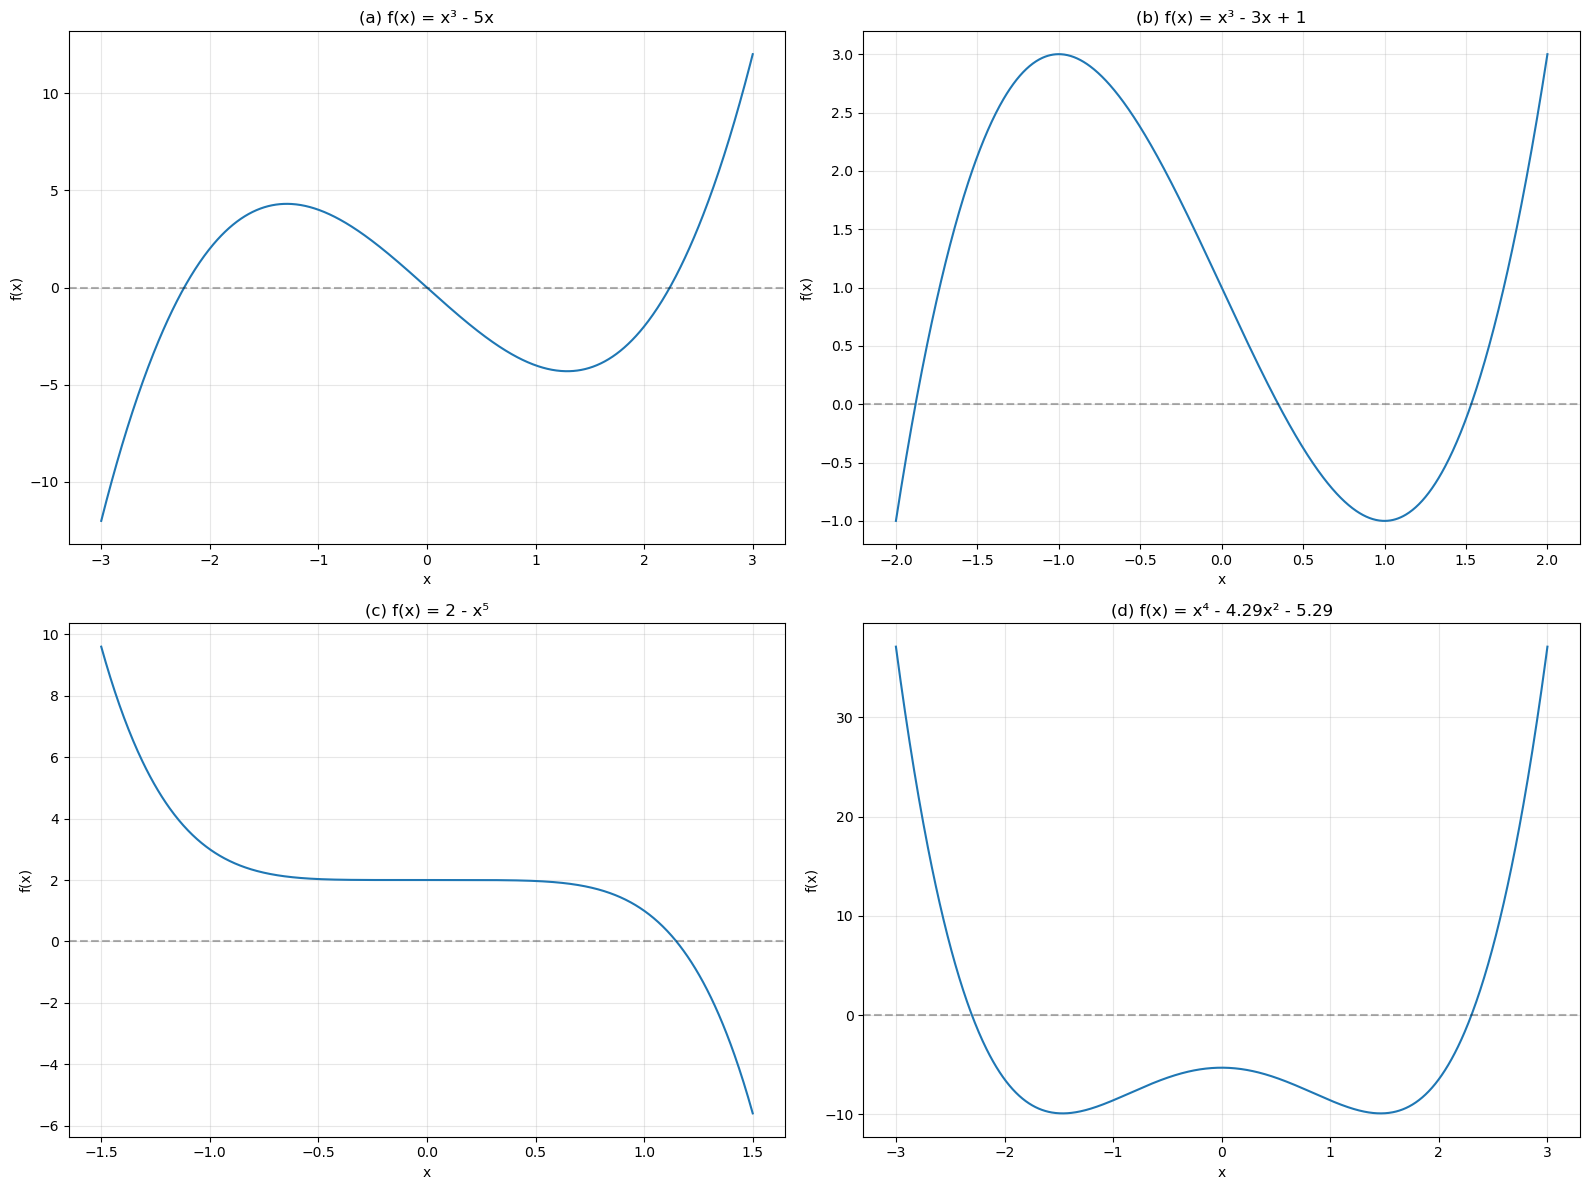
\includegraphics[keepaspectratio]{mownit_lab08_files/figure-pdf/cell-3-output-1.png}}

\begin{verbatim}
Próba metody Newtona i bisection jako zapasowa:

(a)
Newton FAIL: Failed to converge after 50 iterations, value is 1.0.
Newton OK z nowym punktem: znaleziono pierwiastek x = 2.23606797749979

(b)
Newton FAIL: Derivative was zero. Failed to converge after 1 iterations, value is 1.0.
Newton OK z nowym punktem: znaleziono pierwiastek x = 1.532088886237956

(c)
Newton FAIL: Failed to converge after 50 iterations, value is 713.6238464957056.
Newton OK z nowym punktem: znaleziono pierwiastek x = 1.148698354997035

(d)
Newton FAIL: Failed to converge after 50 iterations, value is 0.7876130494100906.
Newton OK z nowym punktem: znaleziono pierwiastek x = 2.3
\end{verbatim}

\subsection{Zadanie 2.}\label{zadanie-2.}

Dane jest równanie:

\(f(x) = x^2 - 3x + 2 = 0\)

Każda z następujących funkcji definiuje równoważny schemat iteracyjny:

\(\phi_1(x) = (x^2 + 2)/3\)

\(\phi_2(x) = \sqrt{3x - 2}\)

\(\phi_3(x) = 3 - 2/x\)

\(\phi_4(x) = (x^2 - 2)/(2x - 3)\)

\begin{itemize}
\tightlist
\item
  Przeanalizuj zbieżność oraz rząd zbieżności schematów iteracyjnych
  odpowiadających funkcjom \(\phi_i(x)\) dla pierwiastka \(\alpha = 2\)
  badając wartość \(|\phi_i'(2)|\).
\item
  Potwierdź analizę teoretyczną implementując powyższe schematy
  iteracyjne i weryfikując ich zbieżność (lub brak). Każdy schemat
  iteracyjny wykonaj przez 10 iteracji. Wyznacz eksprymentalnie rząd
  zbieżności każdej metody iteracyjnej ze wzoru \$ r =
  \frac{\ln \frac{\varepsilon_k}{\varepsilon_{k+1}} }{\ln \frac{\varepsilon_{k-1}}{\varepsilon_k}}\$
  gdzie błąd bezwzględny \(\varepsilon_k\) definiujemy jako
  \(\varepsilon_k=|x_k-x_*|\), \(x_k\) jest przybliżeniem pierwiastka w
  k-tej iteracji, a \(x_*\) dokładnym położeniem pierwiastka równania.
\item
  Na wspólnym rysynku przedstaw wykresy błędu względnego każdej metody w
  zależności od numeru iteracji. Użyj skali logarytmicznej na osi y
  (pomocna będzie funkcja \(\texttt{semilogy}\)).
\item
  Stwórz drugi rysunek, przedstawiający wykresy błędu względnego tylko
  dla metod zbieżnych.
\end{itemize}

\begin{verbatim}
Fixed point iteration results:
\end{verbatim}

\begin{longtable}[]{@{}lllll@{}}
\toprule\noalign{}
& φ\_1(x) & φ\_2(x) & φ\_3(x) & φ\_4(x) \\
\midrule\noalign{}
\endhead
\bottomrule\noalign{}
\endlastfoot
Iteration 0 & 3.000000e+00 & 3.000000 & 3.000000 & 3.000000 \\
Iteration 1 & 3.666667e+00 & 2.645751 & 2.333333 & 2.333333 \\
Iteration 2 & 5.148148e+00 & 2.436648 & 2.142857 & 2.066667 \\
Iteration 3 & 9.501143e+00 & 2.304332 & 2.066667 & 2.003922 \\
Iteration 4 & 3.075724e+01 & 2.216528 & 2.032258 & 2.000015 \\
Iteration 5 & 3.160026e+02 & 2.156289 & 2.015873 & 2.000000 \\
Iteration 6 & 3.328655e+04 & 2.113970 & 2.007874 & 2.000000 \\
Iteration 7 & 3.693315e+08 & 2.083725 & 2.003922 & 2.000000 \\
Iteration 8 & 4.546858e+16 & 2.061838 & 2.001957 & 2.000000 \\
Iteration 9 & 6.891304e+32 & 2.045853 & 2.000978 & 2.000000 \\
Iteration 10 & 1.583003e+65 & 2.034099 & 2.000489 & 2.000000 \\
\end{longtable}

\begin{verbatim}
Experimental convergence orders:
\end{verbatim}

\begin{longtable}[]{@{}lllll@{}}
\toprule\noalign{}
& φ\_1(x) & φ\_2(x) & φ\_3(x) & φ\_4(x) \\
\midrule\noalign{}
\endhead
\bottomrule\noalign{}
\endlastfoot
Iteration 1 & 1.2450 & 0.8947 & 0.7712 & 1.4650 \\
Iteration 2 & 1.3652 & 0.9226 & 0.8995 & 1.7604 \\
Iteration 3 & 1.5478 & 0.9429 & 0.9525 & 1.9586 \\
Iteration 4 & 1.7789 & 0.9577 & 0.9769 & 1.9986 \\
Iteration 5 & 1.9508 & 0.9686 & 0.9886 & NaN \\
Iteration 6 & 1.9973 & 0.9766 & 0.9943 & NaN \\
Iteration 7 & 2.0000 & 0.9826 & 0.9972 & NaN \\
Iteration 8 & 2.0000 & 0.9870 & 0.9986 & NaN \\
Iteration 9 & 2.0000 & 0.9903 & 0.9993 & NaN \\
\end{longtable}

Pochodne funkcji definiujących schematy iteracyjne:

\(|\phi_1'(2)| = 4/3\)

\(|\phi_2'(2)| = 3/5\)

\(|\phi_3'(2)| = 1/2\)

\(|\phi_4'(2)| = 0\)

Powyższe pochodne są mniejsze od 1, oprócz pochodnej \(\phi_1\), dlatego
pozostałe schematy powinny być zbieżne. I tak jest w istocie. Schemat
iteracyjny \(\phi_1\) jest rozbieżny, natomiast pozostałe są zbieżne do
wartości \(x=2\).

Jeśli chodzi o rząd zbieżności, metody 1. i 4. mają rząd zbieżności
równy 2, czyli są kwadratowe. Metody 2. i 3. mają empiryczny rząd
zbieżności równy 1.

\pandocbounded{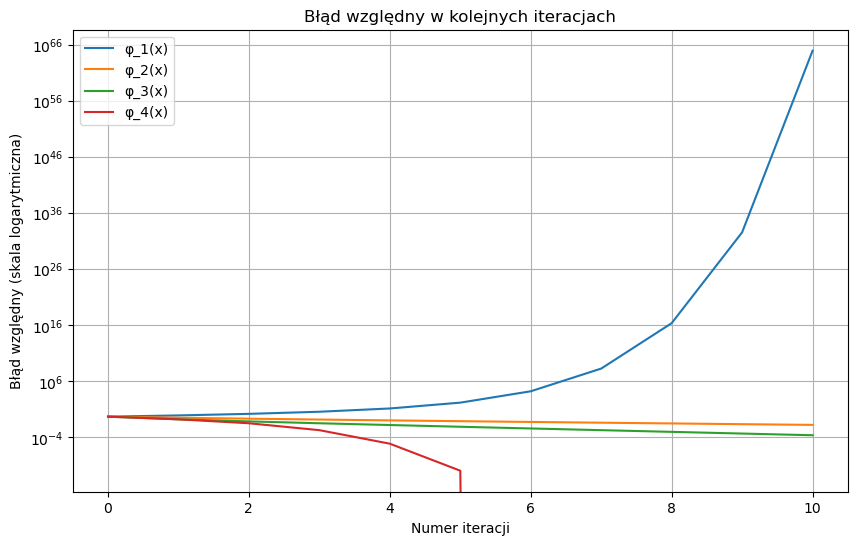
\includegraphics[keepaspectratio]{mownit_lab08_files/figure-pdf/cell-6-output-1.png}}

\pandocbounded{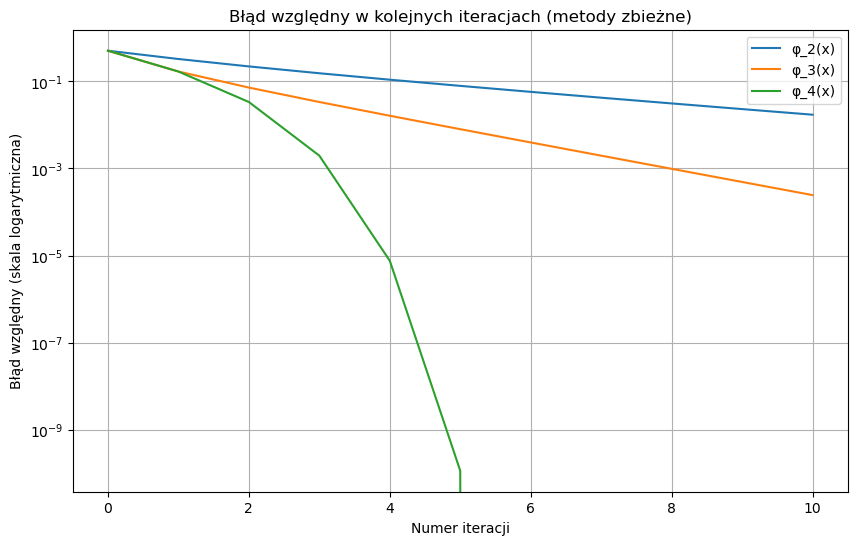
\includegraphics[keepaspectratio]{mownit_lab08_files/figure-pdf/cell-6-output-2.png}}

Powyżej przedstawione są wykresy błędów względnych w kolejnych krokach
iteracyjnych.

Wyraźnie widać, że metoda 4. ma rząd zbieżności większy od liniowego.

\subsection{Zadanie 3.}\label{zadanie-3.}

Napisz schemat iteracji wg metody Newtona dla każdego z następujących
równań nieliniowych:

\begin{enumerate}
\def\labelenumi{\alph{enumi})}
\item
  \(x^3 - 2x - 5 = 0\)
\item
  \(e^{-x} = x\)
\item
  \(x\sin(x) = 1\).
\end{enumerate}

\begin{verbatim}
Rozwiązania 4bit:
\end{verbatim}

\begin{longtable}[]{@{}lll@{}}
\toprule\noalign{}
& x0 4bit & Liczba iteracji \\
\midrule\noalign{}
\endhead
\bottomrule\noalign{}
\endlastfoot
f1 & 2.094568 & 2 \\
f2 & 0.567143 & 2 \\
f3 & 1.114157 & 2 \\
\end{longtable}

\begin{verbatim}
Rozwiązania 24bit:
\end{verbatim}

\begin{longtable}[]{@{}lll@{}}
\toprule\noalign{}
& x0 24bit & Liczba iteracji \\
\midrule\noalign{}
\endhead
\bottomrule\noalign{}
\endlastfoot
f1 & 2.094551 & 2 \\
f2 & 0.567143 & 2 \\
f3 & 1.114157 & 1 \\
\end{longtable}

\begin{verbatim}
Rozwiązania 53bit:
\end{verbatim}

\begin{longtable}[]{@{}lll@{}}
\toprule\noalign{}
& x0 53bit & Liczba iteracji \\
\midrule\noalign{}
\endhead
\bottomrule\noalign{}
\endlastfoot
f1 & 2.094551 & 3 \\
f2 & 0.567143 & 3 \\
f3 & 1.114157 & 1000 \\
\end{longtable}

Dla wszystkich schematów iteracyjnych poza f3 dla 53 bitów, bardzo
szybko zostały osiągnięte docelowe dokładności, dla f3 53 bity nie
została osiągnięta docelowa dokładność w 1000 iteracjach, czyli zapewne
nie zostanie ona osiągnięta.

\section{Zadanie 4.}\label{zadanie-4.}

Napisz schemat iteracji wg metody Newtona dla następującego układu
równań nieliniowych:

\[ x_1^2 + x_2^2 = 1 \] \[ x_1^2 - x_2 = 0 \] Korzystając z faktu, że
dokładne rozwiązanie powyższego układu równań to:
\[ x_1 = \pm \sqrt{\frac{\sqrt{5}}{2} - \frac{1}{2}} \quad \]
\[ x_2 = \frac{\sqrt{5}}{2} - \frac{1}{2} \] oblicz błąd względny
rozwiązania znalezionego metodą Newtona

\begin{verbatim}
Wyniki dla rozwiązania z dodatnim x1:
Wartość teoretyczna: x1 = 0.78615138, x2 = 0.61803399
Wartość numeryczna (metoda Newtona): x1 = 0.78615138, x2 = 0.61803399
Błąd względny składowej x1: 0.00000000e+00
Błąd względny składowej x2: 1.79637859e-16

Wyniki dla rozwiązania z ujemnym x1:
Wartość teoretyczna: x1 = -0.78615138, x2 = 0.61803399
Wartość numeryczna (metoda Newtona): x1 = -0.78615138, x2 = 0.61803399
Błąd względny składowej x1: 0.00000000e+00
Błąd względny składowej x2: 1.79637859e-16
\end{verbatim}

W obu przypadkach obliczone wartości są prawie identyczne - różnica
występuje dopiero na szesnastym miejscu po przecinku. W przypadku
pierwiastka \(x_1\) algorytm znalazł pierwiastek dodatni, ponieważ obie
podane wartości są prawidłowymi rozwiązaniami.




\end{document}
